{\bf BME154L - Spring 2012 - Exam \#2 Solutions}\hfill Name (Net ID):\underline{\hspace*{3.0in}}



%\section{[60 points]}
%
Rectangular waves can be generated from sinusoidal input signals.
Figure~\ref{fig:sine_rect}(b) shows a desired rect output signal that has
asymmetric positive and negative values (-2 and 3 V).

\begin{figure}[htb!]
    \centering
  \begin{tabular}{cc}
    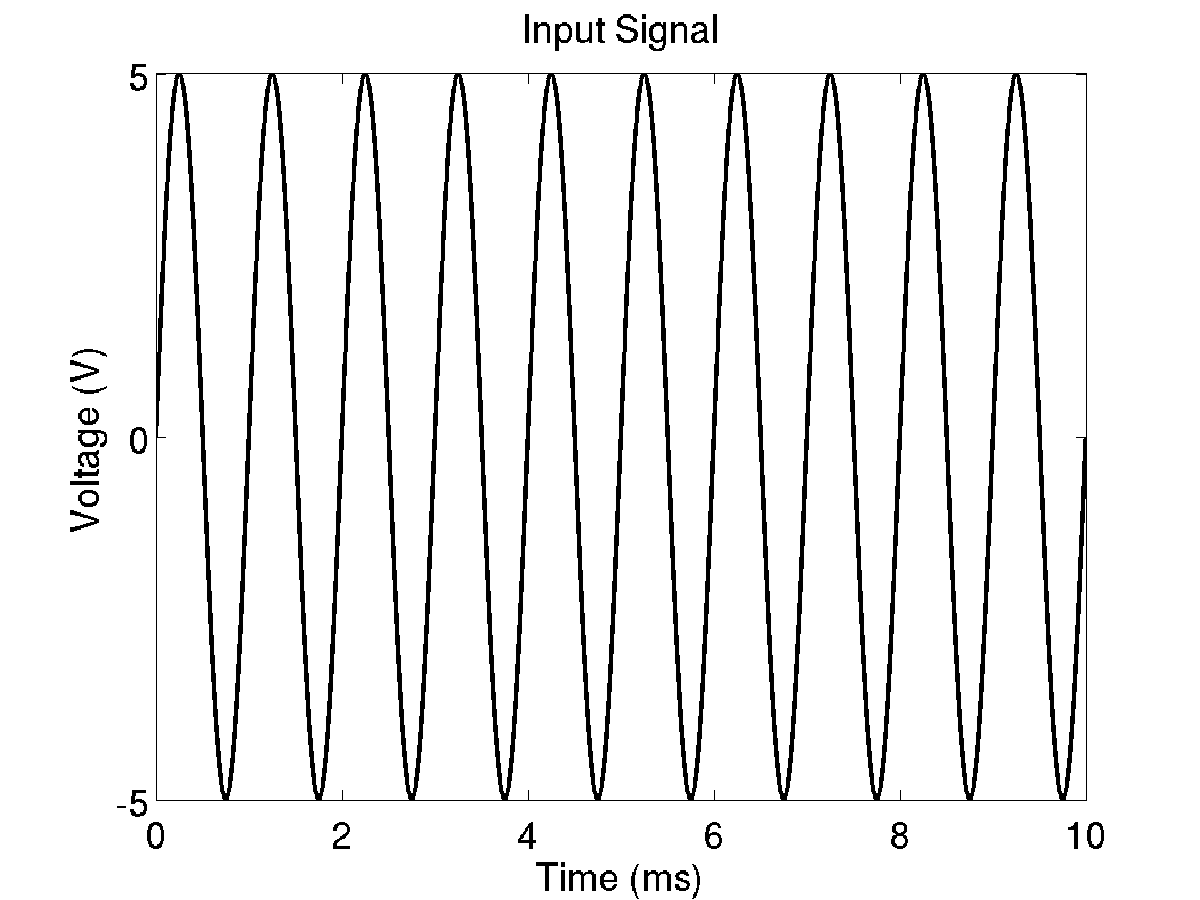
\includegraphics[width=0.4\linewidth]{sine_to_rect/sine_in.png} &
    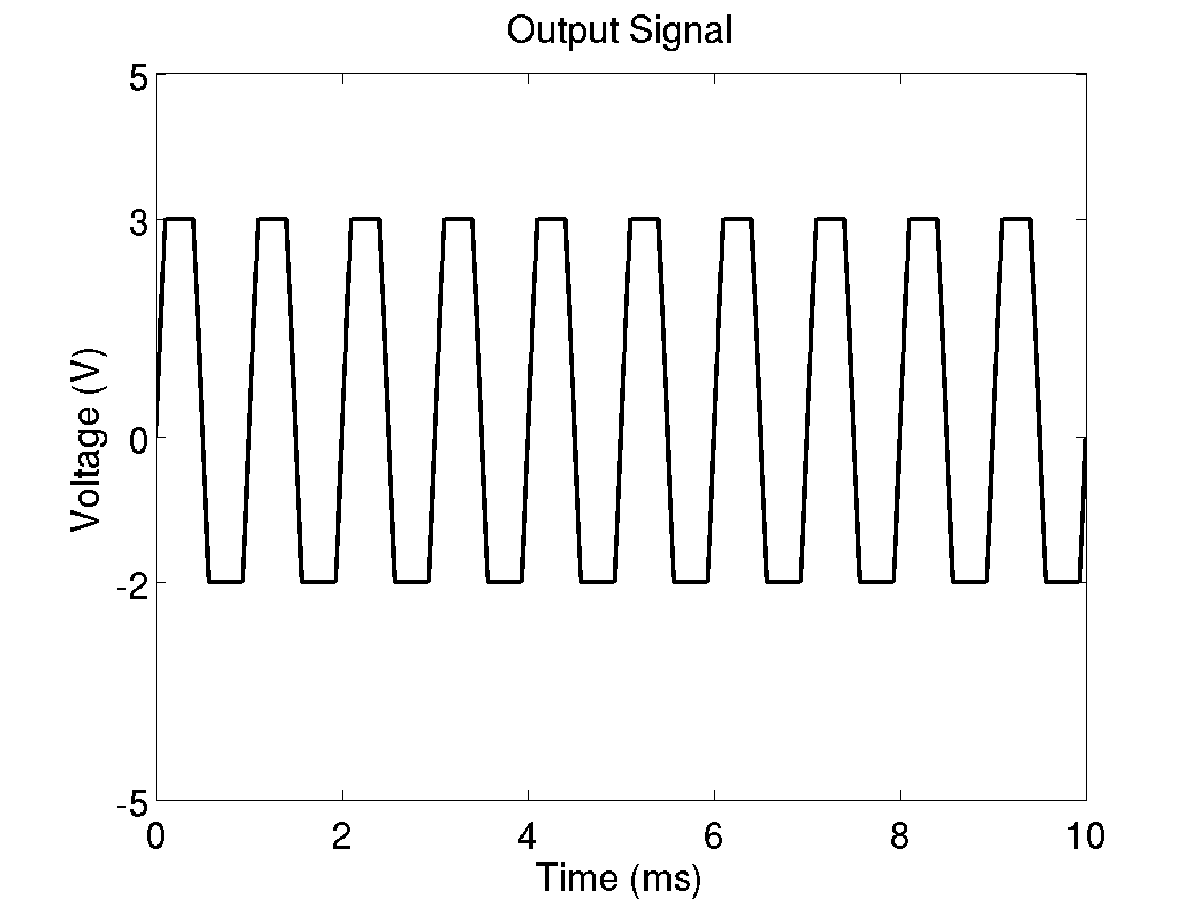
\includegraphics[width=0.4\linewidth]{sine_to_rect/rect_out.png} \\
    (a) Input Signal & (b) Output Signal \\
  \end{tabular}
  \caption{Input and Output Signals}
  \label{fig:sine_rect}
\end{figure}

\begin{enumerate}
  \item Assuming that you have a voltage source ($V_\textrm{in}$) that
    generates the waveform in Figure~\ref{fig:sine_rect}(a), design a
    diode-based circuit to generate the output in
    Figure~\ref{fig:sine_rect}(b).  Assume that any diodes that you use in your
    circuit have forward-bias threshold voltages of 0.7 V. [10 points]

  \item Does the output signal have more or less bandwidth than the input
    signal?  Why? [10 points]

  \item You can also achieve the output signal from $V_\textrm{in}$ by limiting
    the maximum and minimum voltages represented in the analog-to-digital
    conversion process (saturating the ADC).  Design a 3-bit flash ADC that
    limits the digital representation of the sinusoidal input to -2:3 V.
    Please specify all resistor values and, if any, power supplies that you need
    in your circuit, and assume that any op amps that you use rail at
    $\pm$ 12 V.  For now, you can simply represent your priority encoder for
    this ADC as a functional block. [15 points]

  \item What is the SNR of your digitized output signal, expressed in
    dB?\footnote{Remember that in this case, the ``noise'' is related to the
    fact that your output signal is now represented by discrete values.} [5
    points]

  \item The inputs to your priority encoder are expected to be well-conditioned
    logic levels (0 or 5 V).  Given that your op amps being used in your ADC
    rail at $\pm$ 12 V, you will need to ``level shift'' those voltages to 0
    and 5 V.  Design a level shifting circuit that would be used on the output
    of each op amp that shifts -12 V $\rightarrow$ 0 and +12 V $\rightarrow$ 5 V.
    Please specify all relevant component values. [10 points]

  \item The priority encoder in your circuit converts your level-shifted op amp
  outputs to a 3-bit binary number.  This can be achieved with simple logic
  gates (e.g., AND, OR, XOR, etc.).  Designing a priority encoder for a 3-bit
  ADC can be a bit cumbersome during a time-limited exam, so design a priority
  encoder using simple logic gates that would be used for a 2-bit flash ADC.
  ({\it Hint: one simple design could use just 2 OR gates}) [10 points]  

\item What is the minimum sampling frequency ($fs_{min}$) that should be
  used by your ADC to properly capture the frequency content of the input
  signal? [5 points]

\clearpage
{\bf BME154L - Spring 2012 - Exam \#2 Solutions}\hfill Name (Net ID):\underline{\hspace*{3.0in}}



\item Assuming that your input signal runs continuously through time, sketch
  the power spectrum of your sampled input signal when sampled at $fs_{min}$ for a
  frequency range of 0--20 kHz.  On the same sketch, represent the power
  spectrum of your input signal when sample at $2 \times fs_{min}$. Make sure
  that you label which parts of your sketch correspond to each sampling rate.
  [10 points]

\item The Arduino UNO Rev 3 that you will be using for your final projects has
  $\sim$32 kB of flash RAM and can sample data at 10,000 samples / second.
  Given the bit depth of your flash ADC, if you sampled your input signal at
  this maximum sampling rate of the Arduino, then how many seconds of ADC
  output could you store in the Arduino's flash RAM?  How many more
  seconds of data can your store if you sample the input signal at
  $fs_{min}$?  [10 points]

\item Design a DAC that will convert the 3-bit digital representation of the
  output signal to an analog voltage signal without any phase distortion.  You
  can choose any type of DAC, just be sure to specify all relevant component
  values. [15 points]
\end{enumerate}
